\documentclass[main.tex]{subfiles}
\begin{document}
\section{语言及架构}
由于FOC算法为机器人工程中最底层的算法,并且以极高的频率(15$\sim$35kHz)在运行,所以为了提高代码执行效率,在编写代码时应该采用低级语言,大部分FOC代码都使用了C语言(汇编更会获得大家的赞叹)。

本人所写的FOC代码架构共分为$3\sim 4$个层级, 分别为Bsp层、Algorithm层、Task层和Config层(参数过多时单列,参数不多或无需使用flash时省略)。这四个层级的关系如图\ref{代码结构}所示:
\begin{figure}[H]
    \centering
    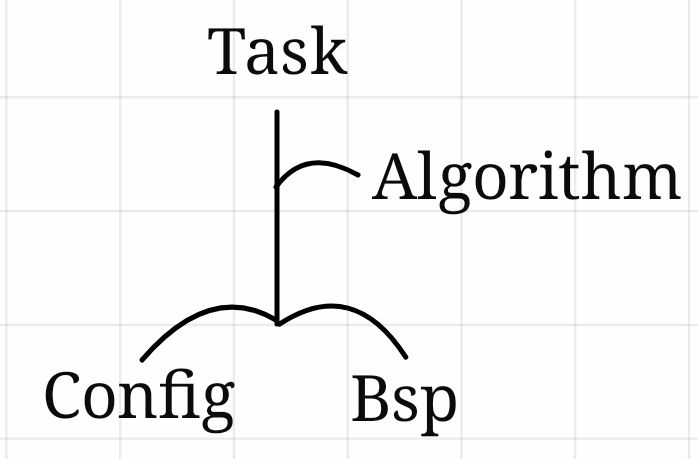
\includegraphics[width=0.3\textwidth]{img/img_1.1.3.png}
    \caption{代码结构}
    \label{代码结构}
\end{figure}

其中Task层包含三个任务,分别为High Freq Task(高频任务),Medium Freq Task(中频任务)和Safety Task(安全任务)。

高频任务的执行频率为20kHz,执行ADC采样,传感器数据解算和FOC任务,并且置标志位使FOC在每次传感器数据解算完成之后运行一次。

中频任务的执行频率为1kHz,执行状态机切换任务,在本任务中判断电机是否使能及其工作模式(电压开环、力矩模式、速度模式、位置模式、混合模式等),并且极易扩展,后续可加无极旋转、拨轮模式等类似Surface Dial的工作模式(纯娱乐)。

安全任务的执行频率为1kHz,用于报警电机异常状态和停止电机的异常工作。由于本电机只有一个LED,所以仅能凭借一个LED的不同闪烁频率报警,而LED又被封死在电机里,所以该任务的功能之一的重点在其可扩展性(高情商发言);当传感器反馈的电机某些状态(母线电压、温度等)超过了电机的合理范围,安全任务将强行令电机停止工作。

Algorithm层为算法层,前述的FOC算法和PID算法及基础数学库包含各种滤波算法在本层中。当算法层验证完成后,不建议修改算法层的任何代码。

Config层为参数层,在本人所写代码中主要包含参数写入flash,参数从flash读出和参数恢复默认操作,也可以将所有define的参数合并为一个.h文件写入本层中(大部分情况下是如此)。在本层中,不建议修改其中代码(除添加参数外)。

Bsp层为板级支持包,主要包含与Hal库直接相关的功能,如串口通信、CAN通信、flash读写、ADC采样、LED闪烁等。本层应该在开始做功能前被验证,验证无误后禁止改动本层代码。同时,Bsp层的存在方便了日后他人的阅读和维护,使代码编写者自己和他人在调试时都能够放下底层与硬件有关的功能,专注上层机器人功能。



\end{document}